\documentclass[espaco=simples,appendix=Name]{abnt}
\usepackage[utf8]{inputenc}
\usepackage[brazil]{babel}
\usepackage{hyperref}
\usepackage[alf]{abntcite}
\usepackage{mdwlist}
\usepackage{dsfont}
\usepackage{graphicx}
\usepackage{placeins}
\def\Data$#1 #2 #3${#2}

\autor{Matheus Eduardo B. Morais e Bruno Rubin}
\titulo{Suporte a Codificação e Decodificação do WebP no Mozilla Firefox}
\orientador{Isabel H. Manssour}
\instituicao{Pontifícia Universidade Católica do Rio Grande do Sul (PUCRS)}
\local{Porto Alegre}
\data{\Data$Date: 2012/12/03 $}


\begin{document}

\capa
\folhaderosto
\listoffigures
\listoftables

\sumario

\newcommand{\ingles}[1]{\textsl{#1}}
\newcommand{\bibTeX}{bib\kern-.13ex\TeX}

\begin{resumo}
Este trabalho tem como objetivo embasar o desenvolvimento do suporte à codificação e decodificação do formato de imagem WebP dentro do navegador Mozilla Firefox. O texto descrito aqui se divide basicamente em quatro partes principais onde a primeira é uma introdução e contextualização do cenário atual, a fundamentação teórica para o projeto, um detalhamento do formato WebP e finalmente a proposta para execução do trabalho. Ao final existem considerações finais a respeito das dificuldades encontradas durante a elaboração deste documento.
\end{resumo}

\begin{abstract}
This paper work have as it main target to base the development of the support to encode and decode the WebP image format inside Mozilla Firefox web browser. The text described here basically organizes in four main sections where the first is an introduction and an contextualization of the current scenario, the theoretical foundation to the project, an close look on WebP format details and finally the proposal to the work execution. At the end there is the final remarks about difficulties found during the creation of this document.
\end{abstract}

\onehalfspacing

\chapter{Introdução}

\section{Contextualização}

Uma tecnologia importante da comunicação utilizada nos dias de hoje dentro da internet é a chamada WWW, ou \ingles{World Wide Web} onde usuários acessam páginas da \ingles{Web} escritas em uma linguagem específica definida por uma organização internacional (W3C), que é renderizada através de um software chamado de navegador. O usuário então pode ler as informações descritas ali e acessar os demais conteúdos da página através de seus hiperlinks de uma maneira fácil e intuitiva.

Com a crescente evolução dos meios de comunicação, a necessidade de total interatividade do usuário com as páginas aumenta cada vez mais. Uma página da \ingles{Web} não é somente texto como era nos primórdios, ela é composta de uma série de diferentes atores como folhas de estilo, imagens e vídeos. Estes atores existem para aumentar a facilidade no uso e causar uma experiência mais agradável para o usuário final.

Apesar da mudança na necessidade dos usuários da \ingles{Web}, nenhuma alteração realmente significativa foi feita no protocolo HTTP cuja última revisão (1.1) ocorreu no ano de 1999 e na linguagem HTML que sofreu seu último ajuste em maio de 2000. Essencialmente a tecnologia implementada atualmente é a mesma criada no início dos anos 90 e apesar de sofrerem pequenas revisões pós criação, continuam não atendendo totalmente as demandas que surgem. Um fator que comprova este fato é a diversidade de tecnologias paralelas (\ingles{plugins}) não oficiais que foram criadas para preencher estas lacunas, o \ingles{Flash}, o \ingles{JavaFX} e o \ingles{Silverlight} são algumas das tecnologias que ilustram este cenário. Outro fator importante é que mesmo com o advento nas tecnologias de comunicação, nem todas as pessoas tem acesso a esta evolução. Seja por uma questão econômica ou mesmo pela falta de infraestrutura, nem toda população do planeta pode contar com aquilo que há de mais moderno.

Recentemente a empresa estadunidense \ingles{Google Inc.} promoveu uma série de iniciativas em conjunto com a comunidade internacional no esforço chamado de "\ingles{Let's make the Web Faster}" \cite{WebFaster}, que consiste em um processo de reengenharia dos protocolos, linguagens e demais itens que compõem a \ingles{Web}. Dentro deste processo novos padrões e formatos estão sendo sugeridos para melhorar a performance e a qualidade na experiência do usuário com as páginas. Uma das sugestões é a utilização de um novo método para compressão de imagens chamado de \ingles{WebP}. Este formato é capaz de comprimir aproximadamente 39\% mais que a melhor solução utilizada hoje que é o formato JPEG \cite{WebPStudy}. O suporte a renderização de imagens \ingles{WebP} está implementado hoje para os navegadores Chrome e Opera.

\section{Motivação}

Os estudos mais recentes mostram que a capacidade de compressão do formato \ingles{WebP} tem cerca de 39\% de ganho quando comparado com JPEG e JPEG200, como pode-se observar na figura a seguir:

\begin{figure}[h]
  \centering
    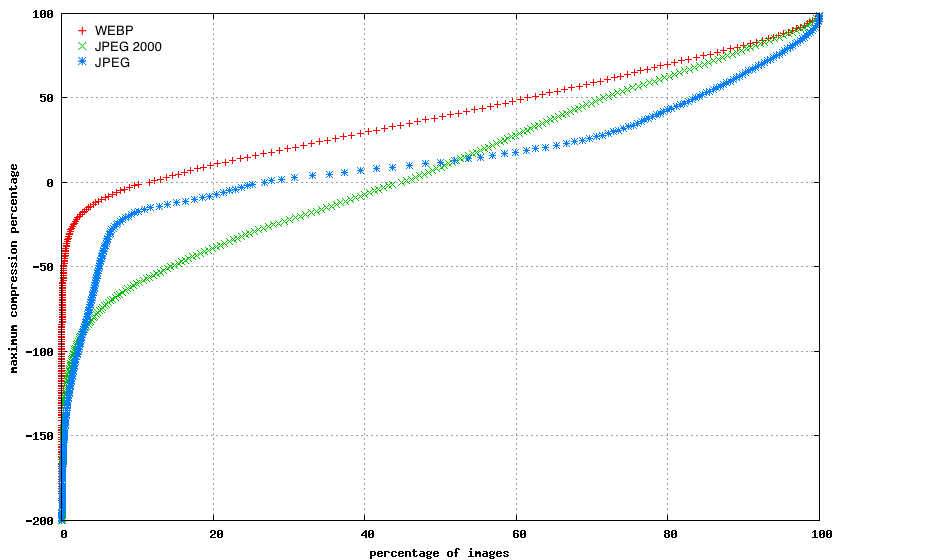
\includegraphics[scale=0.4]{Plot3_cdfcompr.png}
  \caption{Comparação do tamanho das imagens e porcentagem de compressão \protect\cite{WebPStudy}}
\end{figure}

Embora a implementação do suporte ao \ingles{WebP} esteja somente disponível para dois navegadores (Chrome e Opera), estes constituem mais de 29\% de todos os navegadores utilizados dentro da internet hoje. Se houvesse suporte ao \ingles{WebP} dentro do Mozilla Firefox este percentual aumentaria para 52\%, já que cerca de 22\% dos navegadores utilizados hoje são Mozilla Firefox \protect\cite{BrowserStats}, como ilustra a Figura 1.2.

\begin{figure}[h]
  \centering
    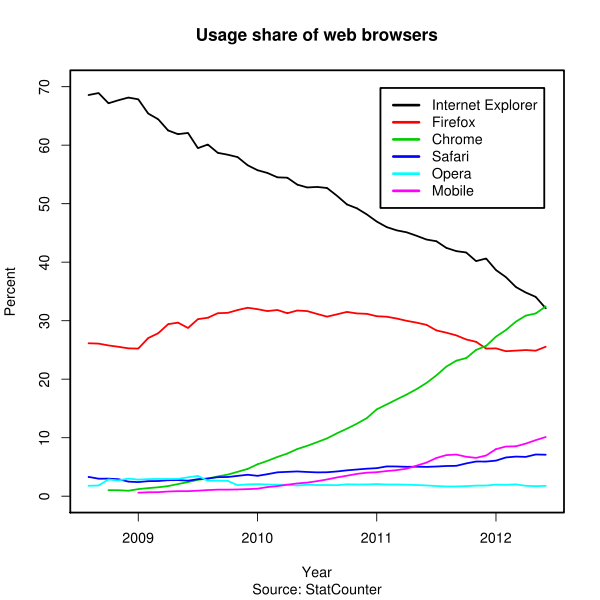
\includegraphics[scale=0.5]{BrowserCounter.png}
  \caption{Percentual de utilização dos Navegadores na Web \cite{BrowserStats}}
\end{figure}

Apesar de não existir nenhuma diretiva da W3C para qual método de compressão de imagens utilizar por padrão, e não se sabe se haverá tal tipo de registro neste sentido no futuro, é importante ressaltar que quanto mais navegadores suportarem a compressão usando o formato \ingles{WebP}, mais os desenvolvedores vão optar por utilizar este formato dada suas vantagens. Uma força de 52\% de suporte dentro dos navegadores da internet também fará com que aqueles que ainda não decidiram pela implementação do suporte ao novo formato, também o façam em virtude da pressão exercida pela maioria.

O aumento na capacidade de compressão do formato \ingles{WebP} trará de imediato a melhora no tempo de resposta para o \ingles{download} da imagem no navegador do usuário, visto que o tamanho dos arquivos será reduzido, e também diminuirá o trafego na comunicação entre cliente e servidor. É importante notar que a utilização em massa deste novo formato vai ajudar na diminuição do trafego de rede dentro da internet de uma maneira global, e isso resulta diretamente em maior vazão para outros recursos que consomem mais banda, como é o caso de um \ingles{streaming} de vídeo por exemplo.

\section{Objetivo}

Com o objetivo de aumentar a disseminação do novo formato dentro da \ingles{Web}, a proposta é de habilitar o suporte de codificação e decodificação do formato WebP dentro do Mozilla Firefox. Embora a implementação do suporte ao \ingles{WebP} esteja somente disponível para dois navegadores (Chrome e Opera), estes constituem mais de 29\% de todos os navegadores utilizados dentro da internet hoje. A implementação do suporte ao \ingles{WebP} dentro do Mozilla Firefox aumentará este percentual para 52\%, já que cerca de 22\% dos navegadores utilizados hoje são Mozilla Firefox \cite{BrowserStats}.

O objetivo deste trabalho não visa a aceitação por parte da equipe do Mozilla, em integrar a implementação desenvolvida ao código fonte do repositório oficial do Firefox. O objetivo é somente contribuir no desenvolvimento para que a renderização nativa do formato WebP seja implementada dentro do navegador. O trabalho desenvolvido poderá ser entregue à comunidade do Firefox, mas sua aplicação oficial na árvore da Mozilla não é o alvo principal. A proposta é a inclusão do suporte à codificação e decodificação do formato de imagem \ingles{WebP} no navegador Mozilla Firefox.


\chapter{Fundamentação Teórica}

\section{A World Wide Web}

A internet hoje em dia se fundamenta nos princípios da \ingles{World Wide Web} ou somente \ingles{Web} como é conhecida. Os usuários se conectam na rede mundial de computadores e utilizam as páginas da \ingles{Web} para realizar todo e qualquer tipo de ação dentro da rede, desde conversar com seus amigos e familiares até realizar compras em uma página de \ingles{e-commerce}.

A \ingles{World Wide Web} foi inventada no CERN (Centro Europeu de Pesquisa Nuclear), com principal objetivo de servir como suporte para a consulta e comunicação interna dos projetos de pesquisa\cite{WebStory}. A ideia inicial era utilizar hipertextos, os quais funcionariam também como hiperlinks e fariam ligações para demais páginas contendo outro tipo de informação. Toda plataforma desenvolvida internamente dentro do CERN para a \ingles{Web} foi posteriormente disponibilizada ao domínio público, sem cobrança de royalties sob qualquer parte. Mais tarde Tim Berners-Lee, o fundador da \ingles{Web} dentro do CERN, criou a o \ingles{World Wide Web Consortium} com o intuito de definir padrões de utilização e interoperabilidade entre tecnologias dentro da rede. Conhecido também como W3C, é composto por funcionários de diversas empresas que trabalham em período integral para manter e evoluir os padrões especificados pela organização \cite{W3Cfacts}.

Além de ser utilizada por pessoas, a \ingles{Web} também é utilizada para comunicação entre sistemas. Efetivamente são computadores acessando outros computadores para realizarem a troca de informações, podendo ser em tempo real ou não. Como os padrões definidos tem suas especificações abertas, a \ingles{Web} também se torna uma ótima ferramenta para integrar sistemas diferentes em plataformas diferentes. Hoje em dia os chamados \ingles{Web-Services} são utilizados juntamente com os conceitos de Orientação a Objetos para integração entre sistemas. A comunicação utilizando os \ingles{Web-Services} se baseia nos princípios e padrões especificados pelo W3C para a \ingles{Web} \cite{WebServices}.

Uma parte importante da \ingles{Web} são os chamados \ingles{Web Browsers} ou Navegadores que servem para que as páginas da \ingles{Web} possam ser acessadas e operadas. Os navegadores são ferramentas que interpretam os padrões descritos pela W3C e fazem a interface para que os humanos consigam entender as informações descritas nas páginas e consigam navegar por elas de forma intuitiva, utilizando os hiperlinks.

Com o advento da qualidade na comunicação da internet, as páginas da \ingles{Web} se tornaram cada vez mais elaboradas e interativas. Atualmente elas não são mais compostas apenas de hipertextos com hiperlinks, esses componentes simples deram espaço para um conjunto de maior complexidade que inclui o processamento de imagens, vídeos e sons. Embora estas funcionalidades dinâmicas existam, não há um padrão claro a respeito delas. A HTML, que é a linguagem de programação da Web, não oferece suporte nativo para todas estas implementações, e plugins adicionais não padronizados são utilizados para implementar estas necessidades específicas (o Flash Player e o Java FX são um exemplo).

A W3C trabalha em uma evolução da linguagem HTML mais preparada para este tipo de cenário, a chamada HTML5. Dentro da HTML5 existem vários detalhes em discussão e um dos mais importantes é a questão da forma como vídeo e imagem serão interpretados. O valor 5 da HTML vem por essa ser a quinta revisão completa da linguagem, que promete ser uma das maiores revisões feitas até hoje \cite{HTML5spec}.


\section{Navegadores}

Com a explosão do uso da \ingles{World Wide Web} na década de 90 \cite{BloombergGameChangers}, diversas grandes empresas da computação, como Microsoft, Google e Apple, investiram no desenvolvimento de novos softwares que possibilitassem aos usuários a busca de dados e informações que estivessem publicadas na Internet. Na computação, um navegador, também chamado de \ingles{Web Browser}, é um \ingles{software} com uma interface gráfica que possui como principal funcionalidade a apresentação de documentos virtuais da Internet, popularmente chamado de páginas da \ingles{Web}.

O navegador é, talvez, o software mais amplamente utilizado na história e teve uma evolução significativa nos últimos quinze anos. Hoje em dia, usuários dos mais variados níveis, utilizam navegadores em diversos tipos de \ingles{hardware}, desde celulares e \ingles{tablets} até computadores comuns \cite{ArchitectureWebBrowsers}.

De acordo com as estatísticas de mercado apresentadas na Tabela 2.1, os navegadores mais utilizados mundialmente são: Opera (Opera Software), Safari (Apple), Internet Explorer (Microsoft), Firefox (Mozilla Corporation \% Mozilla Foundation) e Chrome (Google), em ordem crescente de popularidade \cite{W3schools}.

\begin{table}[ht]
	\centering
	\caption{Estatísticas de utilização dos Navegadores por mês \cite{W3schools}.
	\label{tbl:padc}}{
		\vspace{0.3cm}
		\begin{tabular}{|l|l|l|l|l|l|}
	    	\hline
			\textbf{2012} & \textbf{Internet Explorer} & \textbf{Firefox} &\textbf{Chrome} & \textbf{Safari} & \textbf{Opera} \\
			\hline
			September	& 16.4\% & 32.2\% & 44.1\% & 4.2\% & 2.1\% \\
			\hline
			August		& 16.2\% & 32.8\% & 43.7\% & 4.0\% & 2.2\% \\
			\hline
			July		& 16.3\% & 33.7\% & 42.9\% & 3.9\% & 2.1\% \\
			\hline
			June		& 16.7\% & 34.4\% & 41.7\% & 4.1\% & 2.2\% \\
			\hline
			May			& 18.1\% & 35.2\% & 39.3\% & 4.3\% & 2.2\% \\
			\hline
			April		& 18.3\% & 35.8\% &	38.3\% & 4.5\% & 2.3\% \\
			\hline
			March		& 18.9\% & 36.3\% &	37.3\% & 4.4\% & 2.3\% \\
			\hline
			February	& 19.5\% & 36.6\% &	36.3\% & 4.5\% & 2.3\% \\
			\hline
			January		& 20.1\% & 37.1\% &	35.3\% & 4.3\% & 2.4\% \\
			\hline
		\end{tabular}
		}
\end{table}

A principal funcionalidade de um navegador é apresentar ao usuário o recurso da \ingles{Web} que ele escolher. Este  recurso geralmente é um documento em formato HTML, podendo ser também uma imagem, um arquivo PDF ou outro formato. A localização do recurso é especificada pelo usuário através de uma URL (\ingles{Uniform Resource Locator}), a qual é traduzida pelo navegador e utilizada para realizar a solicitação das informações para um servidor web e posteriormente, exibi-las em sua janela \cite{ArchitectureWebBrowsers}. Um exemplo deste fluxo é apresentado na Figura 2.1.

\begin{figure}[h]
  \centering
    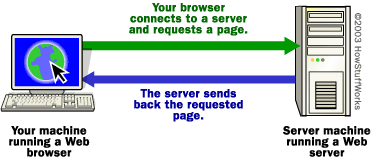
\includegraphics[scale=1]{web_basic.png}
  \caption{Fluxo básico de requisição de uma página da \ingles{Web} para um servidor.}
\end{figure}
 
A forma com que o navegador interpreta e exibe arquivos HTML (\ingles{HiperText Markup Language}) e folhas de estilo CSS (\ingles{Cascading Style Sheet}) são especificações mantidas pela W3C.

A interface gráfica de um navegador possui diversos elementos que são comuns, independente do software que esteja sendo utilizado. Entre estes elementos, pode-se citar: 
\begin{itemize}
	\item Barra de endereços para digitação de URL;
	\item Botão de Home para levar o usuário para a página inicial;
	\item Botões de Voltar e Avançar para as páginas que já foram visualizadas;
	\item Botão de Favoritos;
	\item Botão de Atualizar e Parar, para atualizar e cancelar, respectivamente, o carregamento de páginas.
\end{itemize}

A concorrência existente entre as empresas e os produtos oferecidos atualmente, se dá principalmente pela velocidade de navegação e a utilização dos recursos computacionais. A cada dia, surgem novos padrões e estudos de novas tecnologias relacionadas, que possibilitam que os navegadores tenham um melhor desempenho na execução das suas funções. Um exemplo é o HTML5, que tem como objetivo tornar o conteúdo das páginas mais dinâmico, deixando de lado o conceito do \ingles{browser} que apenas realiza a apresentação do documento, mas que interaja como uma aplicação única através dos recursos e ferramentas \cite{WebAppPlataform}.

\section{HTML5}

Em 1998 o W3C decidiu que eles não iriam mais continuar o desenvolvimento da linguagem da \ingles{Web} até então, a HTML \ingles{(HyperText Markup Language)}. Ao invés disto eles iriam trabalhar em um novo formato o qual acreditavam ser o futuro da \ingles{Web}, assim nasceu a linguagem XHTML \ingles{(Extensible HyperText Markup Language)} que se fundamentava nos princípios da XML \ingles{(Extensible Markup Language)}. Desta forma a revisão 4.01 da HTML foi congelada, e os esforços se direcionaram para a evolução da XHTML que em sua versão 2.0 trazia além de muitas mudanças revolucionárias, a quebra de toda compatibilidade das aplicações escritas nas versões anteriores da especificação.

Muitos não gostaram desta nova iniciativa, em particular um grupo que trabalhava no desenvolvimento do navegador Opera. Estes indivíduos não se convenceram que o XML seria o futuro, e além de não adotar a XHTML, começaram a trabalhar na especificação de uma linguagem HTML extensiva que não quebrasse a compatibilidade das versões anteriores. Este grupo é conhecido como WHATWG (\ingles{Web Hypertext Application Technology Working Group}). A especificação foi inicialmente chamada de \ingles{Web Forms} 2.0 e mais tarde foi nomeada para HTML5 por ser a quinta revisão da HTML \cite{HTML5Intro}. O W3C, então, adotou a versão do grupo WHATWG como base para a nova versão do HTML e começou a trabalhar na quinta revisão, e apesar de não ter sido lançada nenhuma versão final da especificação, praticamente todos navegadores já implementam o suporte à nova definição da HTML. Este processo de desenvolvimento da nova versão passou a ser desenvolvida simultaneamente, pelo W3C e o grupo WHATWG.

Por trás do HTML5 há uma série de princípios de design definidos. De uma forma resumida, pode-se citar três principais princípios\cite{HTML5Intro}:
\begin{itemize}
		\item Interoperabilidade entre os navegadores - Possuir o mesmo comportamento em todos os navegadores, independente de plataforma e tecnologia;
		\item Definição de tratamento de erros - Maneira que os navegadores devem reagir à marcações inválidas;
		\item Evoluir a linguagem para facilitar a criação de conteúdo \ingles{Web}.
\end{itemize}

O HTML5 possui como paradigma ser "livre" de \ingles{plugins}, que são considerados atualmente como os vilões dos navegadores. Os \ingles{plugins}, apesar de adicionar novos elementos e componentes ao navegador, trazem consigo uma série de problemas:

\begin{itemize}
		\item \ingles{Plugins} nem sempre podem ser instalados;
		\item \ingles{Plugins} podem ser desativados ou bloqueados;
		\item \ingles{Plugins} comprometem a segurança e são alvos de ataques;
		\item \ingles{Plugins} são difíceis de integrar ao resto do conteúdo HTML.
\end{itemize}

Os \ingles{plugins} muitas vezes também apresentam dificuldades de integrar seus recursos com o resto do conteúdo exibido pelo navegador, o que acarreta em problemas na renderização do documento. Isto ocorre porque os plugins utilizam um modelo de processamento à parte do qual é utilizado para a página \ingles{Web}. Neste ponto que o HTML5 propões melhorias, trazendo estes recursos de forma nativa na linguagem. Ao invés de utilizar elementos de estilo no formato CSS e \ingles{scripts} com JavaScript, o HTML5 apresenta recursos que não existiam nas versões anteriores. Não são apenas novos elementos que fornecem novas funcionalidades, mas a interação nativa com \ingles{scripts} e estilos que possibilita fazer muito mais do que antes.

Uma das necessidades que a HTML5 deve suprir é o suporte para processamento de vídeo e som que nos dias de hoje se fundamenta no \ingles{plugin Aobe Flash}. Para esta implementação foi escolhido o formato WebM que possibilita aos navegadores renderizar nativamente vídeo e áudio sem a necessidade de instalações adicionais. O formato WebM é composto pelo método de compressão de vídeo VP8 e o padrão de áudio Vorbis. O WebP é parte integrante do WebM, porém, com foco voltado para compressão de imagens.

\chapter{WebP}

\section{Introdução}

O WebP é um novo formato de imagem que implementa compressão \ingles{lossless} e \ingles{lossy} para imagens na \ingles{Web}. Na computação a compressão \ingles{lossless} é aquela que permite a exata reconstrução de uma informação original a partir da informação comprimida, já a compressão \ingles{lossy} é aquela onde porções da informação original são descartadas (perdidas) para que haja efetivamente a compressão. Desta forma, a compressão \ingles{lossy} é utilizada para situações onde a integridade da informação não é exatamente necessária, como é o caso de imagens, vídeo e áudio. Utilizando uma técnica de compressão \ingles{lossless} o WebP consegue apresentar imagens 26\% menores no tamanho quando comparado com o formato PNG. Utilizando imagens com \ingles{lossy} os resultados são ainda melhores, reduz de 25 a 34\% o tamanho da imagem quando comparado com o formato JPEG. Ele também fornece suporte à transparência com apenas 22\% de \ingles{bytes} adicionais. O WebP utiliza uma metodologia semelhante aquela usada na compressão VP8 que faz parte do pacote WebM para o processamento de vídeo e áudio \cite{WebPLossyStudy}.

A tecnologia por trás do WebP é fundamentada no conceito de \ingles{block prediction}. Cada bloco tem seu valor previsto baseando-se nos três blocos acima dele e no primeiro bloco a esquerda dele. Existem quatro métodos para previsão dos blocos, a horizontal, a vertical, a DC e a \ingles{TrueMotion}. As informações que foram previstas incorretamente e os blocos que não são previsíveis são comprimidos em um sub-bloco de 4x4 \ingles{pixels}. No final o resultado é comprimido utilizando \ingles{Entropy encoding}, que é um método \ingles{lossless} amplamente usado para compressão de dados.

O suporte à codificação e decodificação do WebP está disponível nos navegadores Google Chrome e Opera. Como o Mozilla Firefox já possui suporte ao WebM, alguma parte do código para a implementação do WebP já reside dentro do navegador uma vez que tanto WebP quanto VP8 utilizam a mesma técnica para a compressão de imagens pois, no caso de vídeo, o mesmo conceito é utilizado para compressão dos \ingles{frames}.

\section{Mozilla Firefox e o WebP}

O formato WebP foi disponibilizado em 2010 mas nunca conseguiu ser integrado ao Mozilla Firefox. Inclusive na época um \ingles{bug} foi aberto dentro do \ingles{bugzilla} da Mozilla solicitando a implementação do formato WebP \cite{FirefoxBug}. Naquele tempo a equipe principal de desenvolvimento do Mozilla Firefox decidiu por não realizar a implementação em virtude de uma série de considerações contrárias ao formato WebP \cite{WebPCritica}. O time de desenvolvimento do WebP levou em conta as críticas que recebeu dos desenvolvedores do Mozilla Firefox e fez uma série de ajustes para suprir as necessidades que estavam sendo demandadas. Embora praticamente todos os apontamentos dados tenham sido ajustados, ainda não há uma clara razão do por que ele ainda não foi implementado. Em 2010 um \ingles{patch} rudimentar foi escrito e submetido por um membro da comunidade, mas não foi aceito. Existem também algumas extensões que fazem com que o Firefox consiga exibir imagens WebP, porem estas extensões não caracterizam um desenvolvimento adequado visto que elas dependem de \ingles{plugins} adicionais. A proposta é que o navegador seja capaz de realizar a renderização nativamente.

Pelo que se pode averiguar, parece que há por trás disso uma razão política na não adoção do formato WebP até o presente momento. Apesar do Google ter aumentado os investimentos no desenvolvimento do Mozilla Firefox em 2011, o Google Chrome vem tomando espaço do Firefox na internet e há um temor de que a própria existência do Firefox esteja ameaçada graças ao grande sucesso do navegador concorrente. Entretanto pelo que foi pesquisado dentro da comunidade há alguma chance de que caso uma boa implementação seja feita, ela poderá ser aceita dentro do código oficial.

\section{Especificação do Container WebP}

Como um formato de imagem, o WebP utiliza um \ingles{container} RIFF (\ingles{Resource Interchange File Format}) para armazenamento das informações necessárias para utilização do formato dentro de um arquivo. O \ingles{container} do WebP também oferece como característica o suporte para a compressão \ingles{lossless} e o efeito de transparência que pode ser obtido através de um canal \ingles{alpha}. De forma geral o arquivo WebP é composto da imagem representada por uma matriz de \ingles{pixels} no formato VP8 e opcionalmente a informação em relação a transparência.

Basicamente, existem três tipos de arquivos: o formato simples com compressão \ingles{lossy}, o formato simples com a compressão \ingles{lossless} e o formato estendido. Em todos os três tipos existe o cabeçalho do arquivo, que é composto inicialmente pelos caracteres 'RIFF' em ASCII, seguido da informação em relação ao tamanho do arquivo em \ingles{bytes} e por último os caracteres 'WEBP' em ASCII.

\newpage

A figura 3.1 ilustra o formato simples com compressão \ingles{lossy}, o formato simples com a compressão \ingles{lossless} e o formato estendido, respectivamente.

\begin{figure}[h]
  \centering
    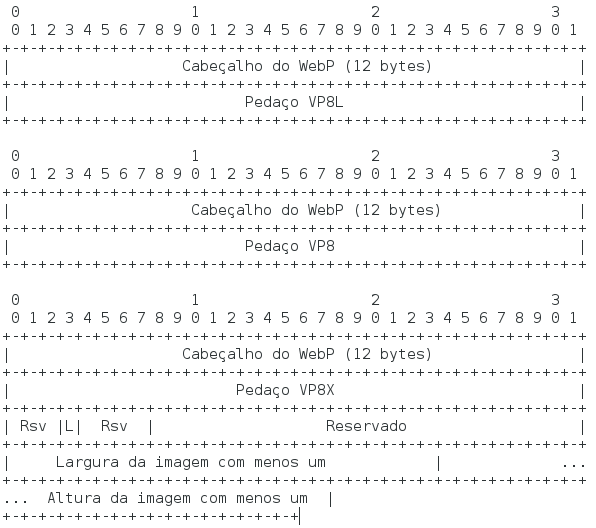
\includegraphics[scale=0.5]{LossyLossLessExtended.png}
  \caption{Formato simples com compressão \ingles{lossy}, formato simples com a compressão \ingles{lossless} e formato estendido}
\end{figure}

A diferença nos formatos simples com compressão \ingles{lossy} e \ingles{lossless} está no pedaço VP8 que por padrão faz a compactação com perda de dados, enquanto que o pedaço VP8L utiliza a compactação sem perda. Já o formato estendido é composto por um pedaço VP8X, mais a informação do canal \ingles{alpha} (L) e o \ingles{bitstream} VP8 ou VP8L. Caso o \ingles{bit alpha} seja setado com valor 1 no formato estendido, sera acrescentado um pedaço adicional para a transparência, como mostra a figura 3.2.

\begin{figure}[h]
  \centering
    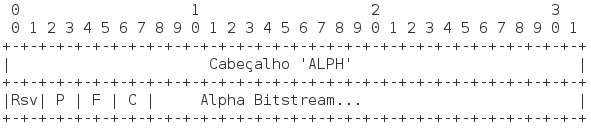
\includegraphics[scale=0.4]{AlphaChunk.png}
  \caption{Pedaço que é acrescentado quando o \ingles{bit alpha} é definido para 1}
\end{figure}

\section{A API libwebp}

A equipe de desenvolvimento do WebP mantém uma biblioteca chamada libwebp que oferece suporte para a criação de ferramentas para a manipulação do formato. No que tange a este trabalho, serão utilizadas as bibliotecas para codificação e decodificação (encode.h e decode.h). Também será necessário utilizar a biblioteca que define os tipos básicos de variáveis e estruturas definidos pelo formato WebP (type.h).

De acordo com a avaliação feita no código fonte e nas definições da biblioteca, as seguintes funções serão utilizadas para criação do decodificador:

\begin{itemize}
	\item WebPGetDecoderVersion
	\item WebPGetInfo
	\item WebPDecodeRGB
	\item WebPDecodeRGBA
	\item WebPDecodeARGB
	\item WebPDecodeBGR
	\item WebPDecodeBGRA
\end{itemize}

As funções utilizadas para criação do codificador serão as seguintes:

\begin{itemize}
	\item WebPGetEncoderVersion
	\item WebPEncodeRGB
	\item WebPEncodeRGBA
	\item WebPEncodeBGR
	\item WebPEncodeBGRA
\end{itemize}

A documentação da biblioteca libwebp é bem simples e direta mas oferece diversos exemplos de utilização, o que a torna bem didática. Nos exemplos criados para este trabalho até o momento, não houve qualquer dificuldade com a utilização das funções e procedimentos definidos pela biblioteca. Os exemplos trabalhados foram a criação de decodificadores e codificadores rudimentares escritos em C++ para o formato WebP com o objetivo de entender melhor como funciona internamente a API. A utilização dela é peça fundamental para implementação do projeto.



\chapter{Trabalhos Relacionados}

Neste capítulo são apresentadas alguns desenvolvimentos e projetos que se assemelham ao assunto deste trabalho, evidenciando soluções distintas e suas características.

\begin{itemize}
%	\item x264 Biblioteca para codificação e decodificação de imagem e áudio.
	\item JPEG 2000 Atualização do padrão JPEG para compressão de imagens.
	\item JPEG XR Alternativa mais leve ao JPEG 2000 para compressão de imagens.
\end{itemize}

%\section{Biblioteca x264}

\section{JPEG 2000}

JPEG 2000 é um padrão de compressão de imagens, criado pela Joint Photographic Experts Group com o objetivo de ser amplamente utilizado em diversas áreas. Suas principais aplicações se deram em câmeras digitais, possibilitando imagens com resoluções maiores, de maior qualidade, utilizando uma compressão dessas informações em um arquivo fisicamente menor; na \ingles{Internet}; em impressões avançadas; em imagens médicas e outros setores chaves. O objetivo do JPEG 2000 não é apenas melhorar o desempenho de compressão em relação ao JPEG, mas adicionar (ou melhorar) características como escalabilidade e capacidade de edição.

O formato JPEG 2000 trouxe alguns benefícios em relação ao JPEG, sendo eles:
\begin{itemize}
	\item Compressão da imagem sem perda de qualidade
	\item Preservação da transparência nas imagens
	\item Uso de máscaras (canais alpha) para especificar uma área da imagem que necessite ser salva em uma taxa de compressão mais baixa (perda de informação de imagem) do que outras áreas que possui um menor interesse para o usuário
	\item Preservação das informações EXIF nos arquivos de imagem
	\item Opções do usuário quanto ao tamanho, qualidade e número de imagem de visualização miniaturas em um site.
\end{itemize}

A principal vantagem oferecida pelo formato JPEG 2000 é a flexibilidade no manuseio do\ingles{codestream} obtido após uma compressão de imagem utilizando este algoritmo. O \ingles{codestream} obtido, pode ser descodificado de diversas maneiras.

O JPEG 2000 foi publicado como um padrão ISO, ISO / IEC 15444. Atualmente o formato não é suportado em navegadores web e, portanto, não é geralmente utilizado na \ingles{Internet}.\cite{JPEG}

\section{JPEG XR}

O formato de imagem JPEG XR (abreviação para \ingles{JPEG extended range}) é um padrão de compressão de imagens desenvolvido e patenteado pela Microsoft sob o nome de HD Photo.
Com a a popularidade do formato JPEG 2000 em baixa, devido à pouco suporte de aplicativos e falta de melhorias no formato, a Microsoft desenvolveu o JPEG XR, na qual se diz comparável com o JPEG 2000, e mais eficiente que o JPEG. Ao contrário do JPEG 2000, este novo formato proposto pela Microsoft é proprietário, ou seja, necessita de drivers e \ingles{plug-ins} específicos para codificação e decodificação das imagens em plataformas que ainda não possui suporte nativo.

O formato JPEG XR suporta a compressão de imagens com e sem perda de qualidade. Em relação ao JPEG original, oferece várias melhorias chave, como:
\begin{itemize}
\item Melhor compressão dos dados
\item Compressão sem perda de qualidade
\item Suporte de cores com maior precisão
\item Suporte a  mapeamento de transparência
\item Suporte a metadados
\end{itemize}

Atualmente o JPEG XR é suportado por diversas aplicações Adobe Flash Player 11.0, Adobe AIR 3.0, Sumatra PDF 2.1, Windows Imaging Component, .NET Framework 3.0, Windows Vista, Windows 7, Windows 8, Internet Explorer 9, Internet Explorer 10, porém não é comumente utilizado em sites da \ingles{Internet}.\cite{HDPhoto}

\chapter{Proposta}

\section{Objetivos}

Conforme apresentado na seção 1.3, o objetivo deste trabalho visa contribuir com o desenvolvimento de uma solução para codificação e decodificação do formato de imagem WebP para o browser Mozilla Firefox. 
Pretende-se, realizar em tempo de execução, a renderização de imagens do formato WebP através da utilização do Mozilla Firefox, possibilitando que o navegador realize a leitura e exibição deste formato de imagem para o usuário. Inicialmente será realizado um estudo da biblioteca do formato WebP, na qual é disponibilizada pelo Google. 
A motivação do desenvolvimento desta solução, conforme descrito na seção 1.2, se dá pelo fato de que o formato WebP já se encontrar em um estado avançado de desenvolvimento e maturidade, e já estar recebendo suporte nativo dos browsers Google Chrome e Opera. 

O aumento na capacidade de compressão do formato \ingles{WebP} trará de imediato a melhora no tempo de resposta para o \ingles{download} da imagem no navegador do usuário e também diminuirá o trafego na comunicação entre cliente e servidor. É importante ressaltar também que a popularização e utilização em massa deste novo formato irá beneficiar na diminuição do trafego de rede dentro da internet de uma maneira global, e isso resulta diretamente em uma vazão maior para outros recursos que consomem mais banda, como é o caso de um \ingles{streaming} de vídeo por exemplo.

No ano de 2010 um \ingles{patch} rudimentar foi escrito e submetido por um membro da comunidade, mas não foi aceito. Existem também algumas extensões que fazem com que o Firefox consiga exibir imagens WebP, porem estas extensões não caracterizam um desenvolvimento adequado visto que elas dependem de \ingles{plugins} adicionais. A proposta é que o navegador seja capaz de realizar a renderização nativamente. Nenhum trecho do \ingles{patch} enviado em 2010 através do \ingles{bug} aberto será aproveitado dentro deste trabalho, será necessário uma produção a partir do zero.

Pelo que se pode averiguar, parece que há por trás disso uma razão política na não adoção do formato WebP até o presente momento. Apesar do Google ter aumentado os investimentos no desenvolvimento do Mozilla Firefox em 2011, o Google Chrome vem tomando espaço do Firefox na internet e há um temor de que a própria existência do Firefox esteja ameaçada graças ao grande sucesso do navegador concorrente. Entretanto pelo que foi pesquisado dentro da comunidade há alguma chance de que caso uma boa implementação seja feita, ela poderá ser aceita dentro do código oficial, embora isto não seja o principal objetivo do trabalho.

Como o tempo para implementação do projeto é reduzido não haverá espaço para a reescrita de uma nova API dentro do Firefox. O que será feito é a incorporação da biblioteca libwebp desenvolvida pelo Google dentro do Firefox e o trabalho efetivamente será a criação do decodificador e codificador integrado com as bibliotecas do próprio Firefox.

\section{Projeto}

Visando atingir os objetivos descritos para este trabalho, foi criado o seguinte cronograma de atividades a ser seguido na disciplina de Trabalho de Conclusão I:
\begin{enumerate}
	\item Estudo do formato WebP e da biblioteca libwebp;
	\item Estudo e análise do código do Mozilla Firefox;
	\item Estudo dos padrões de codificação do Mozilla Firefox;
	\item Estudo da viabilidade de implementação;
	\item Estudo do patch proposto em 2010;
	\item Desenvolvimento da primeira parte da documentação para o trabalho final.
	\item Criação de um \ingles{fork} da última versão do projeto no repositório oficial.
	\item \ingles{Merge} da biblioteca libwebp no código do Mozilla Firefox.
	\item Criação do codificador e decodificador para o formato WebP.
	\item Ajuste no inicializador e carregador das imagens do Mozilla Firefox.
	\item Criação dos arquivos para compilação.
	\item Desenvolvimento da segunda e última parte da documentação para o trabalho final.
\end{enumerate}

\begin{figure}[h]
  \centering
    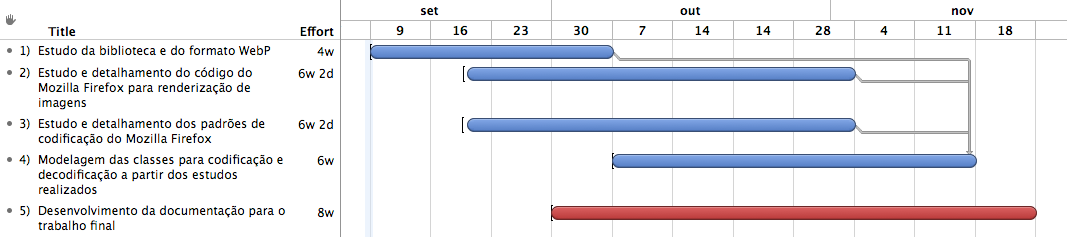
\includegraphics[scale=0.6]{scheduler.png}
  \caption{Cronograma de atividades}
\end{figure}

O planejamento futuro para implementação vislumbra a criação de um \ingles{fork} a partir do projeto atual disponível na árvore oficial do Firefox. O trabalho então será feito em cima deste projeto separado para evitar que as atualizações constantes dos mantenedores atrapalhe o desenvolvimento que será realizado.

\section{Ambiente de Desenvolvimento}

As principais ferramentas utilizadas para o desenvolvimento deste trabalho estão listadas na tabela 5.1.

\begin{table}[ht]
	\centering
	\caption{Ferramentas utilizadas para o desenvolvimento do trabalho.
	\label{tbl:padc}}{
		\vspace{0.3cm}
		\begin{tabular}{|l|p{14cm}|}
	    	\hline
			\textbf{Ferramenta} & \textbf{Descrição} \\
			\hline
			LaTeX		& Conjunto de macros para processamento de texto. Está sendo utilizado para criação de todo material textual. \\
			\hline
			GIT		& Ferramenta utilizada para controle versão distribuída. \\
			\hline
			AbnTeX		& Biblioteca LaTeX para processamento de texto utilizando as normas da ABNT. \\
			\hline
			BibTeX		& Ferramenta utilizada para gerenciamento das referências descritas na documentação. \\
			\hline
			VIM		& Editor de texto. \\
			\hline
			Bash		& Interpretador de comandos que está sendo utilizado para compilação e geração da documentação através de \ingles{scripts}. \\
			\hline
			DIA		& Ferramenta utilizada para o desenho de diagramas. \\
			\hline
		\end{tabular}
		}
\end{table}

\section{Modelagem e Arquitetura}

A arquitetura de desenvolvimento do Mozilla Firefox permite a extensão de funcionalidades na renderização de imagens sem a necessidade de alteração de grandes porções de código já existente. É uma arquitetura bem modular e com baixo acoplamento, o que permite a fácil integração de novos componentes quando necessário. 

De uma maneira geral, o núcleo a ser alterado para implementar a codificação e decodificação do formato WebP é a parte responsável pela inicialização das imagens (Image.h e Image.cpp) e pelo carregamento das imagens (ImageLoader.h e ImageLoader.cpp). Uma vez que o codificador e o decodificador estejam prontos, será necessário fazer alterações neste módulos para que o navegador possa nativamente manipular as imagens no formato WebP. Na figura 5.1 é possível ver um diagrama macro que mostra o nível de alteração necessária nos módulos de imagem e como eles se relacionam entre si.

\begin{figure}[h]
  \centering
    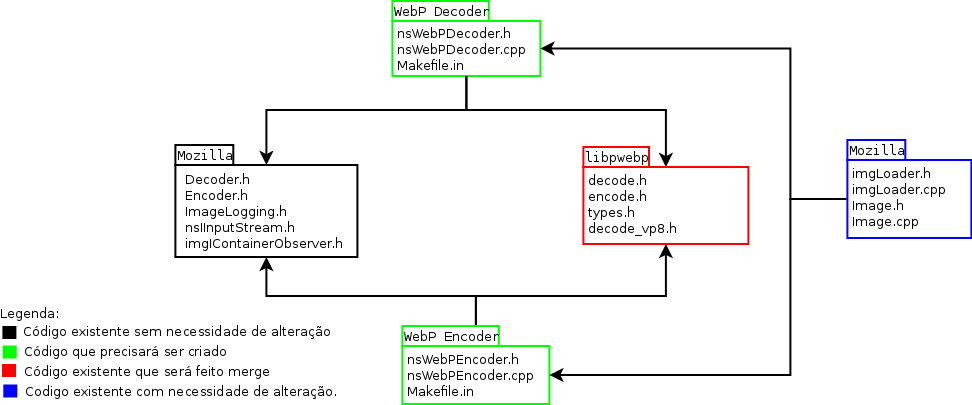
\includegraphics[scale=0.45]{Arquitetura.png}
  \caption{Diagrama dos componentes e suas relações}
\end{figure}

Também serão necessárias pequenas alterações em outros pontos como por exemplo a definição do \ingles{mime-type} para o formato WebP que deve ser acrescentado dentro do Firefox, mas estas não caracterizam mudança significativas de forma que a maior parte do trabalho será realizada em cima do núcleo de manipulação de imagens do navegador, conforme mostrado no diagrama dos componentes.

\chapter{Comentários Finais}

A implementação da codificação e decodificação do formato WebP dentro do navegador Mozilla Firefox se faz possível conforme demonstrado pelo estudo feito na fundamentação teórica, no entendimento do formato propriamente dito e principalmente na descrição do projeto. Apesar de ter uma documentação bastante ampla, a falta de artigos científicos publicados prejudicou a composição das referências deste trabalho. Como a especificação do formato só foi feita e divulgada ao público em meados de 2010 após a compra da empresa On2 pelo Google, é possível que tenha havido pouco tempo para a criação de trabalhos acadêmicos relacionados ao WebP.

Apesar da evolução constante realizada pele equipe de desenvolvimento, existem ainda diversos processos burocráticos pendentes que atrapalham no processo de adoção da tecnologia, como por exemplo o cadastramento do formato dentro de órgãos de registro da internet como a IANA (\ingles{Internet Assigned Numbers Authority}). Sabe-se que a adoção de um formato depende não somente da qualidade da tecnologia, mas sim da amplitude de sua utilização. Por este motivo o seu sucesso está diretamente associado à disseminação da tecnologia tanto por parte dos \ingles{softwares} de manipulação de imagens, quanto pelos navegadores de internet. O formato não pode se mostrar apenas eficiente do ponto de vista de infraestrutura, os desenvolvedores precisam achar atrativos e recursos interessantes para optarem por utilizar o WebP, e esse é um dos maiores desafios que os mantenedores oficiais do formato precisam resolver.

\bibliography{proposta}

\end{document}
